\documentclass{ximera}

%\usepackage{todonotes}

\newcommand{\todo}{}

\usepackage{esint} % for \oiint
\ifxake%%https://math.meta.stackexchange.com/questions/9973/how-do-you-render-a-closed-surface-double-integral
\renewcommand{\oiint}{{\large\bigcirc}\kern-1.56em\iint}
\fi


\graphicspath{
  {./}
  {ximeraTutorial/}
  {basicPhilosophy/}
  {functionsOfSeveralVariables/}
  {normalVectors/}
  {lagrangeMultipliers/}
  {vectorFields/}
  {greensTheorem/}
  {shapeOfThingsToCome/}
  {dotProducts/}
  {partialDerivativesAndTheGradientVector/}
  {../productAndQuotientRules/exercises/}
  {../normalVectors/exercisesParametricPlots/}
  {../continuityOfFunctionsOfSeveralVariables/exercises/}
  {../partialDerivativesAndTheGradientVector/exercises/}
  {../directionalDerivativeAndChainRule/exercises/}
  {../commonCoordinates/exercisesCylindricalCoordinates/}
  {../commonCoordinates/exercisesSphericalCoordinates/}
  {../greensTheorem/exercisesCurlAndLineIntegrals/}
  {../greensTheorem/exercisesDivergenceAndLineIntegrals/}
  {../shapeOfThingsToCome/exercisesDivergenceTheorem/}
  {../greensTheorem/}
  {../shapeOfThingsToCome/}
  {../separableDifferentialEquations/exercises/}
  {vectorFields/}
}

\newcommand{\mooculus}{\textsf{\textbf{MOOC}\textnormal{\textsf{ULUS}}}}

\usepackage{tkz-euclide}
\usepackage{tikz}
\usepackage{tikz-cd}
\usetikzlibrary{arrows}
\tikzset{>=stealth,commutative diagrams/.cd,
  arrow style=tikz,diagrams={>=stealth}} %% cool arrow head
\tikzset{shorten <>/.style={ shorten >=#1, shorten <=#1 } } %% allows shorter vectors

\usetikzlibrary{backgrounds} %% for boxes around graphs
\usetikzlibrary{shapes,positioning}  %% Clouds and stars
\usetikzlibrary{matrix} %% for matrix
\usepgfplotslibrary{polar} %% for polar plots
\usepgfplotslibrary{fillbetween} %% to shade area between curves in TikZ
%\usetkzobj{all}
\usepackage[makeroom]{cancel} %% for strike outs
%\usepackage{mathtools} %% for pretty underbrace % Breaks Ximera
%\usepackage{multicol}
\usepackage{pgffor} %% required for integral for loops



%% http://tex.stackexchange.com/questions/66490/drawing-a-tikz-arc-specifying-the-center
%% Draws beach ball
\tikzset{pics/carc/.style args={#1:#2:#3}{code={\draw[pic actions] (#1:#3) arc(#1:#2:#3);}}}



\usepackage{array}
\setlength{\extrarowheight}{+.1cm}
\newdimen\digitwidth
\settowidth\digitwidth{9}
\def\divrule#1#2{
\noalign{\moveright#1\digitwidth
\vbox{\hrule width#2\digitwidth}}}




% \newcommand{\RR}{\mathbb R}
% \newcommand{\R}{\mathbb R}
% \newcommand{\N}{\mathbb N}
% \newcommand{\Z}{\mathbb Z}

\newcommand{\sagemath}{\textsf{SageMath}}


%\renewcommand{\d}{\,d\!}
%\renewcommand{\d}{\mathop{}\!d}
%\newcommand{\dd}[2][]{\frac{\d #1}{\d #2}}
%\newcommand{\pp}[2][]{\frac{\partial #1}{\partial #2}}
% \renewcommand{\l}{\ell}
%\newcommand{\ddx}{\frac{d}{\d x}}

% \newcommand{\zeroOverZero}{\ensuremath{\boldsymbol{\tfrac{0}{0}}}}
%\newcommand{\inftyOverInfty}{\ensuremath{\boldsymbol{\tfrac{\infty}{\infty}}}}
%\newcommand{\zeroOverInfty}{\ensuremath{\boldsymbol{\tfrac{0}{\infty}}}}
%\newcommand{\zeroTimesInfty}{\ensuremath{\small\boldsymbol{0\cdot \infty}}}
%\newcommand{\inftyMinusInfty}{\ensuremath{\small\boldsymbol{\infty - \infty}}}
%\newcommand{\oneToInfty}{\ensuremath{\boldsymbol{1^\infty}}}
%\newcommand{\zeroToZero}{\ensuremath{\boldsymbol{0^0}}}
%\newcommand{\inftyToZero}{\ensuremath{\boldsymbol{\infty^0}}}



% \newcommand{\numOverZero}{\ensuremath{\boldsymbol{\tfrac{\#}{0}}}}
% \newcommand{\dfn}{\textbf}
% \newcommand{\unit}{\,\mathrm}
% \newcommand{\unit}{\mathop{}\!\mathrm}
% \newcommand{\eval}[1]{\bigg[ #1 \bigg]}
% \newcommand{\seq}[1]{\left( #1 \right)}
% \renewcommand{\epsilon}{\varepsilon}
% \renewcommand{\phi}{\varphi}


% \renewcommand{\iff}{\Leftrightarrow}

% \DeclareMathOperator{\arccot}{arccot}
% \DeclareMathOperator{\arcsec}{arcsec}
% \DeclareMathOperator{\arccsc}{arccsc}
% \DeclareMathOperator{\si}{Si}
% \DeclareMathOperator{\scal}{scal}
% \DeclareMathOperator{\sign}{sign}


%% \newcommand{\tightoverset}[2]{% for arrow vec
%%   \mathop{#2}\limits^{\vbox to -.5ex{\kern-0.75ex\hbox{$#1$}\vss}}}
% \newcommand{\arrowvec}[1]{{\overset{\rightharpoonup}{#1}}}
% \renewcommand{\vec}[1]{\arrowvec{\mathbf{#1}}}
% \renewcommand{\vec}[1]{{\overset{\boldsymbol{\rightharpoonup}}{\mathbf{#1}}}}

% \newcommand{\point}[1]{\left(#1\right)} %this allows \vector{ to be changed to \vector{ with a quick find and replace
% \newcommand{\pt}[1]{\mathbf{#1}} %this allows \vec{ to be changed to \vec{ with a quick find and replace
% \newcommand{\Lim}[2]{\lim_{\point{#1} \to \point{#2}}} %Bart, I changed this to point since I want to use it.  It runs through both of the exercise and exerciseE files in limits section, which is why it was in each document to start with.

% \DeclareMathOperator{\proj}{\mathbf{proj}}
% \newcommand{\veci}{{\boldsymbol{\hat{\imath}}}}
% \newcommand{\vecj}{{\boldsymbol{\hat{\jmath}}}}
% \newcommand{\veck}{{\boldsymbol{\hat{k}}}}
% \newcommand{\vecl}{\vec{\boldsymbol{\l}}}
% \newcommand{\uvec}[1]{\mathbf{\hat{#1}}}
% \newcommand{\utan}{\mathbf{\hat{t}}}
% \newcommand{\unormal}{\mathbf{\hat{n}}}
% \newcommand{\ubinormal}{\mathbf{\hat{b}}}

% \newcommand{\dotp}{\bullet}
% \newcommand{\cross}{\boldsymbol\times}
% \newcommand{\grad}{\boldsymbol\nabla}
% \newcommand{\divergence}{\grad\dotp}
% \newcommand{\curl}{\grad\cross}
%\DeclareMathOperator{\divergence}{divergence}
%\DeclareMathOperator{\curl}[1]{\grad\cross #1}
% \newcommand{\lto}{\mathop{\longrightarrow\,}\limits}

% \renewcommand{\bar}{\overline}

\colorlet{textColor}{black}
\colorlet{background}{white}
\colorlet{penColor}{blue!50!black} % Color of a curve in a plot
\colorlet{penColor2}{red!50!black}% Color of a curve in a plot
\colorlet{penColor3}{red!50!blue} % Color of a curve in a plot
\colorlet{penColor4}{green!50!black} % Color of a curve in a plot
\colorlet{penColor5}{orange!80!black} % Color of a curve in a plot
\colorlet{penColor6}{yellow!70!black} % Color of a curve in a plot
\colorlet{fill1}{penColor!20} % Color of fill in a plot
\colorlet{fill2}{penColor2!20} % Color of fill in a plot
\colorlet{fillp}{fill1} % Color of positive area
\colorlet{filln}{penColor2!20} % Color of negative area
\colorlet{fill3}{penColor3!20} % Fill
\colorlet{fill4}{penColor4!20} % Fill
\colorlet{fill5}{penColor5!20} % Fill
\colorlet{gridColor}{gray!50} % Color of grid in a plot

\newcommand{\surfaceColor}{violet}
\newcommand{\surfaceColorTwo}{redyellow}
\newcommand{\sliceColor}{greenyellow}




\pgfmathdeclarefunction{gauss}{2}{% gives gaussian
  \pgfmathparse{1/(#2*sqrt(2*pi))*exp(-((x-#1)^2)/(2*#2^2))}%
}


%%%%%%%%%%%%%
%% Vectors
%%%%%%%%%%%%%

%% Simple horiz vectors
\renewcommand{\vector}[1]{\left\langle #1\right\rangle}


%% %% Complex Horiz Vectors with angle brackets
%% \makeatletter
%% \renewcommand{\vector}[2][ , ]{\left\langle%
%%   \def\nextitem{\def\nextitem{#1}}%
%%   \@for \el:=#2\do{\nextitem\el}\right\rangle%
%% }
%% \makeatother

%% %% Vertical Vectors
%% \def\vector#1{\begin{bmatrix}\vecListA#1,,\end{bmatrix}}
%% \def\vecListA#1,{\if,#1,\else #1\cr \expandafter \vecListA \fi}

%%%%%%%%%%%%%
%% End of vectors
%%%%%%%%%%%%%

%\newcommand{\fullwidth}{}
%\newcommand{\normalwidth}{}



%% makes a snazzy t-chart for evaluating functions
%\newenvironment{tchart}{\rowcolors{2}{}{background!90!textColor}\array}{\endarray}

%%This is to help with formatting on future title pages.
\newenvironment{sectionOutcomes}{}{}



%% Flowchart stuff
%\tikzstyle{startstop} = [rectangle, rounded corners, minimum width=3cm, minimum height=1cm,text centered, draw=black]
%\tikzstyle{question} = [rectangle, minimum width=3cm, minimum height=1cm, text centered, draw=black]
%\tikzstyle{decision} = [trapezium, trapezium left angle=70, trapezium right angle=110, minimum width=3cm, minimum height=1cm, text centered, draw=black]
%\tikzstyle{question} = [rectangle, rounded corners, minimum width=3cm, minimum height=1cm,text centered, draw=black]
%\tikzstyle{process} = [rectangle, minimum width=3cm, minimum height=1cm, text centered, draw=black]
%\tikzstyle{decision} = [trapezium, trapezium left angle=70, trapezium right angle=110, minimum width=3cm, minimum height=1cm, text centered, draw=black]

\author{Jim Talamo (edited)}

\title{Special Series}



\begin{document}
\begin{abstract}
geometric
\end{abstract}
\maketitle

Suppose that we have a \emph{series} $\sum\limits_{k=k_0}^{\infty} a_k$ and have to determine whether it converges or diverges.  To answer this question, we define a new \emph{sequence} $\{s_n\}_{n=k_0}$ where $s_n = \sum\limits_{k=k_0}^{n}$ for all $n \geq k_0$.  We saw previously that
 
 \begin{itemize}
\item the series $\sum\limits_{k=k_0}^\infty a_k$ \textbf{converges} if and only if $\lim\limits_{n\to\infty} s_n$ exists.  
\item the series $\sum\limits_{k=k_0}^\infty a_k$ \textbf{diverges} if and only if $\lim\limits_{n\to\infty} s_n$ does not exist.  
\end{itemize}

The definitions above give us a way to determine whether a given series converges.  In fact, to determine whether $\sum\limits_{k=k_0}^{\infty} a_k$ converges, we can do the following.

\begin{itemize}
\item Consider the associated sequence $\{s_n\}$ of partial sums.
\item Try to find an explicit formula for the term $s_n$.  If you can find such a formula, analyze $\lim\limits_{n \to \infty} s_n$.  
\begin{itemize}
\item If $\lim\limits_{n \to \infty} s_n$ exists, then $\sum\limits_{k=k_0}^{\infty} a_k$ converges, and if we can determine that $\lim\limits_{n \to \infty} s_n =L$, then $\sum\limits_{k=k_0}^{\infty} a_k=L$.  
\item If  $\lim\limits_{n \to \infty} s_n$ does not exist, then $\sum\limits_{k=k_0}^{\infty} a_k$ diverges.
\end{itemize}
\item  If an explicit formula for $s_n$ cannot be found, further analysis is needed.  
\end{itemize}









\section*{A recursive formula for $s_n$}
The most straightforward way to determine whether $\lim\limits_{n \to \infty} s_n$ exists is to have an explicit formula for the $n$-th term $s_n$.  Note that this is not an easy task; for example, can you find a formula for $s_n$ for the series $\sum\limits_{k=1}^{\infty} \frac{1}{k}$? It's not too hard to write out the first several terms in the sequence $\{s_n\}_{n=1}$, but try to find an explicit formula for $s_n$!

As it turns out, there is always a recursive formula for $s_n$, and this will play an important role in later sections.  Suppose that we want to consider $\sum\limits_{k=1}^{\infty} a_k$.  Let's write out the formula for $s_n$.

\[
s_n = a_1+a_2+a_3+\ldots+a_{n-1}+a_n
\]

We can make an observation by considering $s_{n-1}$ in a similar way.

\[
s_{n-1} = a_1+a_2+a_3+\ldots+a_{n-1}
\]

Now returning to our expression for $s_n$, we can make an observation. 
\begin{image}
  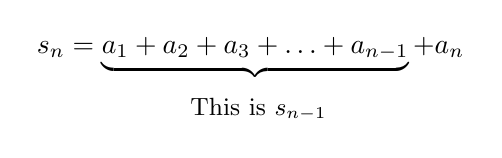
\begin{tikzpicture}
        \node at (0,0) {
          $s_n = \underbrace{a_1+a_2+a_3 + \ldots + a_{n-1}}+ a_n$};
        \node at (.1,-.65) {\small{This is $s_{n-1}$}};
      
      \end{tikzpicture}
  \end{image}

We thus have the formula 

\[
s_n = s_{n-1}+a_n.
\]

If we apply this to the series $\sum\limits_{k=1}^{\infty} \frac{1}{k}$, we have $s_n = \sum\limits_{k=1}^n \frac{1}{k}$ and $a_n = \frac{1}{n}$.  The recursive formula reads 

\begin{align*}
s_n &= s_{n-1} +a_n\\
s_n &= s_{n-1} +  \frac{1}{n}.
\end{align*}

This does not help us analyze whether $\lim\limits_{n \to \infty} s_n$ actually exists.  Sometimes, however, we can find an \emph{explicit} formula for $s_n$, and we study a special type of series for which this is possible.




















\section*{A special types of series : Geometric}



Recall that a \emph{geometric sequence} is a sequence for which the ratio of successive terms is constant.  If $\{a_n\}_{n=n_0}$ is such a sequence, then there are constants $a \ne 0$ and $r$ for which $a_n = a\cdot r^n$.  

We thus represent this sequence by the ordered list

\[
a \, r^{n_0} , a \, r^{n_0+1}, a \, r^{n_0+2}, \ldots
\]

and we have a result that characterizes the behavior of this type of sequence, which we recall now.


\begin{theorem}
  Given a geometric sequence $\{a_n\}_{n=n_0}$ where $a_n = a \cdot r^{n}$,
  \[
  \lim_{n\to\infty} a_n =
  \begin{cases}
    0 &\text{if $|r|<1$,}\\
    a &\text{if $r=1$,}\\
    \text{DNE} &\text{if $|r|>1$ or $r=-1$.}
  \end{cases}
  \]
\end{theorem}

We can now ask when we are able to \textbf{\textcolor{purple!85!blue}{sum}} the terms of a geometric sequence.

\begin{definition}  \textbf{\textcolor{green!50!black}{Geometric Series}} 


  A \textbf{geometric series} is a series of the form $\sum\limits_{k=k_0}^\infty a \, r^k$
  for some real numbers $a \ne 0$ and $r$.
\end{definition}

Before exploring when such a series converges, note that sometimes, some preliminary algebra is necessary to recognize a series as geometric.

\begin{example}
The series $\sum\limits_{k=4}^\infty \frac{2^{2k+1}}{3^k}$ \wordChoice{\choice[correct]{is}\choice{is not}} geometric since $a_k =\frac{2^{2k+1}}{3^k}$ \wordChoice{\choice[correct]{can}\choice{cannot}} be brought into the form $a \cdot r^k$.  

Using the laws of exponents shows us:

\[
\frac{2^{2k+1}}{3^k} = \frac{2^{2k} \cdot 2^1}{3^k}= 2 \cdot \frac{\left(2^{k}\right)^2}{3^k} = 2 \cdot \frac{4^k}{3^k} = 2 \cdot \left(\frac{4}{3}\right)^k.
\]
Indeed, $a= \answer[given]{2}$ and $r = \answer[given]{\frac{4}{3}}$.
\end{example}

\begin{example}
The series $\sum\limits_{k=0}^\infty k^2 \left(\frac{1}{2}\right)^k$ \wordChoice{\choice{is}\choice[correct]{is not}} geometric since $a_k = \answer[given]{k^2 \cdot \frac{1}{2}^k}$ \wordChoice{\choice{can}\choice[correct]{cannot}} be brought into the form $a \cdot r^k$.  Indeed, the coefficient, $k^2$, is not the same for each term in the series.
\end{example}

We can now try to determine when adding together the terms in such a series is possible; that is, we can explore for which values of $a$ and $r$ the \emph{series} $\sum\limits_{k=n_0}^{\infty} a \, r^k$ converges.  










\begin{model}
 Let $r \neq 1$ and consider the geometric series $\sum\limits_{k=0}^\infty a \, r^k$, and let $s_n = \sum\limits_{k=0}^{n} a \, r^k $.  We find an explicit formula for the term $s_n$.
  
  \begin{explanation}
First, note that the sum above represents the attempt to add all of the terms in the sequence $\{a_n\}_{n=0}$, where $a_n =  r^n$.  Let's start by writing out $s_n$.  

    \begin{align*}
      s_n   &= 1 + r + r^2 + \dots + r^n\\
    \end{align*}

The issue with finding a formula for $s_n$ arises from the fact that we cannot perform the above for an unspecified value $n$.  However, to go from one term in the sum to the next, we multiply by $r$, so let's multiply both sides of the above equation by $r$.
    \begin{align*}
      s_n   &= 1 + r + r^2 + \dots + r^n\\
      r s_n &= ~ \phantom{ 1 + } r + r^2 + \dots + r^n + r^{n+1}
    \end{align*}
Now, we can subtract away the middle terms, which we show (with some slight abuse of notation) below.
 \[     \begin{array}{rl}
      s_n   &= 1 + \cancel{ r + r^2 + \dots + r^n}\\
 -\left(  \phantom{ r^{n+1}} r s_n \right.&=~ \left. \phantom{  1 +  } \cancel{r + r^2 + \dots + r^n} + r^{n+1}\right) \\
 \hline 
     s_n - r s_n &= 1 \phantom{  +  r + r^2 + \dots + r^n } ~ - r^{n+1}\\
    \end{array}
 \]   
 We can now solve for $s_n$.
     \begin{align*}
      s_n - r s_n &= 1 - r^{n+1}\\
      s_n(1-r)    &= 1 - r^{n+1}\\
      s_n &= \frac{1 - r^{n+1}}{1-r}.
    \end{align*}
    Since $r \ne 1$, there is no issue dividing by $1-r$; we will treat the case $r=1$ a bit later.
  \end{explanation}
\end{model}








From our work above, we see that the $n$-th partial sum of the
geometric series $a_n = r^n$ is
\[
s_n = \sum\limits_{k=0}^{n} r^k= \frac{1 - r^{n+1}}{1-r}.
\]
We now have an \emph{explicit} formula so we can determine for which values of $r$ the limit $\lim\limits_{n \to \infty} s_n$ exists.  Let's first do a little algebraic thinking, 

\[
\lim\limits_{n \to \infty} s_n = \lim\limits_{n \to \infty}  \frac{1 - r^{n+1}}{1-r} =   \lim\limits_{n \to \infty}  \left( \frac{1}{1-r} - \frac{1}{1-r} \cdot r^{n+1} \right) 
\]


$\frac{1}{1-r}$ has nothing to do with $n$.  Therefore, the limit has nothing to do with this fraction.


\[
=  \frac{1}{1-r}  - \frac{1}{1-r}  \lim\limits_{n \to \infty} r^{n+1}.
\]





The existence of $\lim\limits_{n \to \infty} s_n $ is thus entirely determined by whether $\lim\limits_{n \to \infty} r^{n+1}$ exists, and this limit is the limit of a geometric \emph{sequence}!  In fact, 

\begin{itemize}
\item if $-1<r<1$, then $\lim\limits_{n \to \infty} r^{n+1}$ \wordChoice{\choice[correct]{exists}\choice{does not exist}}. \\
\item if $r>1$ or $r\le -1$, then $\lim\limits_{n \to \infty} r^{n+1}$ \wordChoice{\choice{exists}\choice[correct]{does not exist}}.
\end{itemize}

The above formula covers every case except when $r= 1$, but notice that  $$\sum\limits_{k=0}^n 1 = n+1,$$ so if $r=1$, $s_n = \answer[given]{n+1}$ and $\lim\limits_{n \to \infty} s_n = \infty$, so $\sum\limits_{k=0}^{\infty} 1$ diverges. 

When $-1<r<1$, note $\lim\limits_{n \to \infty} r^{n+1}=0$, so in this case,     \[
    \lim\limits_{n\to\infty}\frac{1 - r^{n+1}}{1-r} = \frac{1-\answer[given]{0}}{1-r}.
    \]

By noting that $\sum\limits_{k=0}^n a \, r^k = a \sum\limits_{k=0}^n r^k$, we can combine this observation with the above argument and write the result in a theorem.

\begin{theorem}
  The geometric series $\sum\limits_{k= 0}^\infty a \cdot r^k$ 
  
  \begin{itemize} 
  \item converges to $\frac{a}{1-r}$ when $|r| < 1$.
  \item diverges if $|r| \geq 1$.  
  \end{itemize}
  \end{theorem}

A little algebra allows us to find the sum of a convergent geometric series when the lower index does not start at $0$.  

\begin{example}
The series $\sum\limits_{k=3}^{\infty} \left(\frac{2}{3}\right)^k$ is a geometric series with $r=\frac{2}{3}<1$, so it converges.  To find the value to which it converges, notice the following.

\begin{align*}
\sum\limits_{k=3}^{\infty} \left(\frac{2}{3}\right)^k &=  \left(\frac{2}{3}\right)^3+ \left(\frac{2}{3}\right)^4+ \left(\frac{2}{3}\right)^5+\ldots \\
&= \left(\frac{2}{3}\right)^3 \cdot \left(1+ \frac{2}{3}+ \left(\frac{2}{3}\right)^2+\ldots\right) \\
&= \frac{8}{27}  \cdot  \sum_{k=0}^{\infty}\left(\frac{2}{3}\right)^k \\
&= \sum\limits_{k=0}^{\infty} \frac{8}{27}  \cdot \left(\frac{2}{3}\right)^k
\end{align*}
This is now a geometric series whose lower index is $0$, so we can use the formula to find its value. Noting that $a=\answer[given]{ \frac{8}{27} }$ and $r= \frac{2}{3}$ gives:

\[
\sum\limits_{k=3}^{\infty} \left(\frac{2}{3}\right)^k = \frac{8/27}{1-2/3} = \frac{8}{9}.
\]
\end{example}

We can easily generalize this example and doing so allows us to write down a more comprehensive theorem about geometric series.

\begin{theorem}
\index{series!geometric}\index{geometric series}\index{geometric series!convergence}\index{geometric series!divergence}
  The geometric series $\sum\limits_{k= k_0}^\infty a \cdot r^k$ 
  
  \begin{itemize} 
  \item converges to $\frac{a \, r^{k_0}}{1-r}$ when $|r| < 1$.
  \item diverges if $|r| \geq 1$.  
  \end{itemize}
  \end{theorem}
 
\begin{example}
Let's take another look at the series that started off the section, $\sum\limits_{k=1}^{\infty} \left(\frac{1}{2}\right)^k$.  Here, $a=\answer[given]{1}$, $r=\answer[given]{1/2}$ and $k_0 = \answer[given]{1}$.  Since $|r|<1$, the series \wordChoice{\choice[correct]{converges}\choice{diverges}}, and using the formula above, we have that

\[ \sum\limits_{k=1}^{\infty} \left(\frac{1}{2}\right)^k = \frac{a \, r^{k_0}}{1-r} = \frac{1\cdot \frac{1}{2}}{1-1/2} =1.\]

This matches the earlier result!  
\end{example}

\begin{remark} 
Although we have mentioned it before, we mention it again here:

\begin{quote}
The lower index in a series does not affect whether the series converges or diverges, but if the series converges, it can affect the value to which the series converges.
\end{quote}
The formula listed above very explicitly shows exactly how the lower index $k_0$ affects the value to which a convergent geometric series converges.

\end{remark}

Now, try some questions to check your understanding of the above material.

\begin{question}
  Which of the following series converge?
  \begin{selectAll}
    \choice{$\sum\limits_{k=0}^\infty \left(\frac{3}{2}\right)^k$}
    \choice[correct]{$\sum\limits_{k=0}^\infty \left(\frac{-2}{3}\right)^k$}
    \choice[correct]{$\sum\limits_{k=9}^\infty \left(\frac{1}{7}\right)^k$}
    \choice{$\sum\limits_{k=1}^\infty (-1)^k$}
    \choice[correct]{$\sum\limits_{k=-9}^\infty \left(\frac{1}{2}\right)^k$}    
  \end{selectAll}
  \begin{hint}
    The initial index doesn't matter as far as convergence is
    concerned, it is the ``tail'' of the sequence that determines
    convergence.
  \end{hint}
\end{question}

\begin{question}
Determine if the series $\sum\limits_{k=2}^{\infty} 2^{3-2k}$ converges or diverges.  If it converges, give the value to which it converges.

\begin{explanation}
First, note that the series \wordChoice{\choice[correct]{is}\choice{is not}} geometric since the laws of exponents allow us to write the following.

\[
2^{3-2k} = \frac{2^3}{2^{2k}} = \frac{8}{\left(2^2\right)^k} =  8 \cdot \frac{1}{4^k} =  8 \cdot \frac{1^k}{4^k} =  8 \cdot \left(\frac{1}{4}\right)^k
\]

The series is geometric with $r = \answer[given]{1/4}$, and using the result $\sum\limits_{k=k_0} a \cdot r^k = \frac{a \, r^{k_0}}{1-r}$ gives:

\[
\sum\limits_{k=2}^{\infty} 2^{3-2k} =  8 \cdot \left(\frac{1}{4}\right)^k =  \frac{8 \cdot (1/4)^2}{1-1/4}  =  \answer[given]{\frac{2}{3}}.
\]
\end{explanation}

\end{question}    


























%%%%%%%%%%%%%%%%%%%%%%%%%%%%%%
\section*{Summary}
Now that we have seen a special type of series for which we can find an explicit formula for the $n$-th term of the sequence of partial sums, it helps to summarize the logic that we employed.

\begin{itemize}
\item[1.] Consider the associated sequence $(s_n)$ of partial sums.
\item[2.] Try to find an explicit formula for the term $s_n$.  If you can find such a formula, analyze $\lim\limits_{n \to \infty} s_n$.  
\begin{itemize}
\item If the limit exists, $\sum\limits_{k=k_0}^{\infty} a_k$ converges, and if we can determine that $\lim\limits_{n \to \infty} s_n =L$, then $\sum\limits_{k=k_0} a_k=L$.  \item If  $\lim\limits_{n \to \infty} s_n$ does not exist, then $\sum\limits_{k=k_0} a_k$ diverges.
\end{itemize}
\end{itemize}
















\begin{center}
\textbf{\textcolor{green!50!black}{ooooo-=-=-=-ooOoo-=-=-=-ooooo}} \\

more examples can be found by following this link\\ \link[More Examples of Sums of Sequences]{https://ximera.osu.edu/csccmathematics/precalculus1/precalculus1/sumsOfSequences/examples/exampleList}

\end{center}






\end{document}
